\begin{knitrout}
\definecolor{shadecolor}{rgb}{1, 1, 1}\color{fgcolor}\begin{kframe}
\begin{alltt}
\hlstd{h_normal} \hlkwb{<-} \hlnum{1.06} \hlopt{*} \hlstd{s} \hlopt{*} \hlstd{n}\hlopt{^}\hlstd{(}\hlopt{-}\hlnum{1} \hlopt{/} \hlnum{5}\hlstd{)}

\hlstd{h} \hlkwb{<-} \hlstd{h_normal}

\hlstd{n_bins} \hlkwb{<-} \hlkwd{floor}\hlstd{(}\hlkwd{diff}\hlstd{(}\hlkwd{range}\hlstd{(x))} \hlopt{/} \hlstd{h)}
\hlstd{f_hist} \hlkwb{<-} \hlkwd{hist}\hlstd{(x,} \hlkwc{breaks} \hlstd{= n_bins,} \hlkwc{plot} \hlstd{=} \hlnum{FALSE}\hlstd{)}
\hlstd{f_epa} \hlkwb{<-} \hlkwd{as.data.frame}\hlstd{(}\hlkwd{bkde}\hlstd{(x,} \hlkwc{kernel} \hlstd{=} \hlstr{"epa"}\hlstd{,} \hlkwc{bandwidth} \hlstd{= h))}

\hlkwd{ggplot}\hlstd{(x_df,} \hlkwd{aes}\hlstd{(x))} \hlopt{+}
 \hlkwd{geom_histogram}\hlstd{(}
   \hlkwd{aes}\hlstd{(}\hlkwc{y} \hlstd{= ..density..),}
   \hlkwc{binwidth} \hlstd{= h,}
   \hlkwc{col} \hlstd{=} \hlstr{"black"}\hlstd{,}
   \hlkwc{fill} \hlstd{=} \hlstr{"white"}
 \hlstd{)} \hlopt{+}
 \hlkwd{stat_function}\hlstd{(}
   \hlkwc{fun} \hlstd{= dnorm,}
   \hlkwc{args} \hlstd{=} \hlkwd{list}\hlstd{(}\hlkwc{mean} \hlstd{= mu,} \hlkwc{sd} \hlstd{= sigma),}
   \hlkwc{color} \hlstd{=} \hlstr{"red"}
 \hlstd{)} \hlopt{+}
 \hlkwd{geom_line}\hlstd{(}\hlkwc{data} \hlstd{= f_epa,} \hlkwd{aes}\hlstd{(x, y),} \hlkwc{color} \hlstd{=} \hlstr{"blue"}\hlstd{)} \hlopt{+}
 \hlkwd{theme_minimal}\hlstd{(}\hlkwc{base_size} \hlstd{=} \hlnum{20}\hlstd{)}
\end{alltt}
\end{kframe}
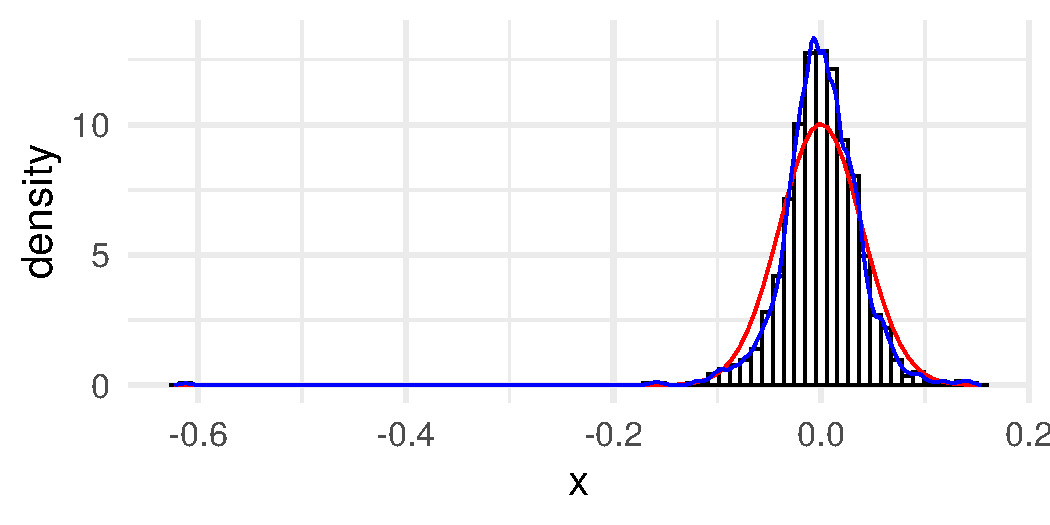
\includegraphics[width=\maxwidth]{figure/unnamed-chunk-23-1} 

\end{knitrout}
